\modeCorrection

%%%% début de la page

\renewcommand{\thesubsection}{\textcolor{red}{\Roman{section}.\arabic{subsection}}}
\renewcommand{\thesubsubsection}{\textcolor{red}{\Roman{section}.\arabic{subsection}.\alph{subsubsection}}}

\setcounter{section}{0}
\setcounter{document}{0}
\sndEnTeteTPSix

\begin{center}
\begin{mdframed}[style=titr, leftmargin=60pt, rightmargin=60pt, innertopmargin=7pt, innerbottommargin=7pt, innerrightmargin=8pt, innerleftmargin=8pt]

\begin{center}
\large{\textbf{TP 6 : Les sodas sont-ils trop sucrés ?
}}
\end{center}
\end{mdframed}
\end{center}

\begin{tableauCompetences}
    APP & Exploiter des explications orales pour rédiger un protocole & & & & \\
    \hline
    REA & Réaliser une série de mesures ; relever les résultats obtenus & & & & \\
     \hline 
     REA & Utiliser une grandeur quotient pour déterminer le numérateur ou le dénominateur& & & & \\
     \hline 
    COM & Rendre compte de façon écrite & & & & \\
    \hline
    VAL & Analyser l’ensemble des résultats de façon critique  & & & &
\end{tableauCompetences}


%%%% objectifs
\begin{tcolorbox}[colback=blue!5!white,colframe=blue!75!black,title=Objectifs de la séance :]
\begin{itemize}
    \item Choisir et utiliser la verrerie adaptée pour préparer une solution par dissolution,
    \item Réaliser une courbe d'étalonnage,
    \item Déterminer la valeur d’une concentration en masse à partir de résultats expérimentaux.
\end{itemize}
\end{tcolorbox}

%%%% Consignes
\begin{tcolorbox}[colback=red!5!white,colframe=red!75!black,title= Consignes :]
\begin{itemize}
    \item Rendre un compte-rendu par binôme en fin de TP,
    \item Faire attention à la verrerie lors de son utilisation,
    \item Respectez les consignes d'utilisation de la salle de chimie.
\end{itemize}
\end{tcolorbox}

%%%% contexte

\begin{tcolorbox}[colback=orange!5!white,colframe=orange!75!black,title= Scénario:]
\begin{wrapfigure}{r}{0.4\textwidth}
\vspace{-0.6cm}
    \centering
      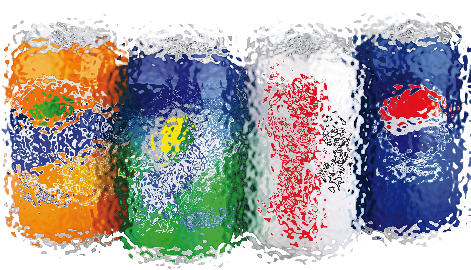
\includegraphics[width=0.4\textwidth]{Images/TP/TP6/Soda_flou.png}
  \end{wrapfigure}
La consommation de soda dans le monde est gigantesque. Pour la marque Coca-cola, des études statistiques estiment que la consommation moyenne de ce soda est d'environ 350 milliards de litres par jour.\\
Les sodas sont des boissons gazeuses pour la plupart très sucrées pouvant causer une maladie qu'on a pu nommer que très récemment : la maladie du soda ou maladie du foie gras. Cette maladie cause des effets très sévères à moyen et long terme : diabète de type 2, excès de graisse dans le foie, ... Une étude pilotée par l'INSERM (Institut National de la Santé et de la Recherche Médicale) a montré que près d’un français sur cinq (18,2\%) présente un excès de graisse dans le foie.

\problematique{Quelle est la concentration en masse de sucre dans une bouteille de soda de marque bien connue ?}
\end{tcolorbox}
\newpage

\begin{mdframed}[style=autreexo]
\textbf{\bsc{Liste du matériel}}
\begin{itemize}
    \item Spatule ;
    \item Balance ;
    \item Fiole jaugée de 100,0 mL ;
    \item Béchers ;
    \item Entonnoir en plastique ;
    \item Une bouteille de soda dégazée ;
    \item Sucre ;
    \item Eau ;
    \item Logiciel tableur-grapheur (Excel) ; 
\end{itemize}
\end{mdframed}

\begin{doc}{\'{E}tiquette d'une bouteille de soda d'une marque bien connue}
\vspace{-0.4cm}
  \label{doc:Coca}
  \begin{center}
     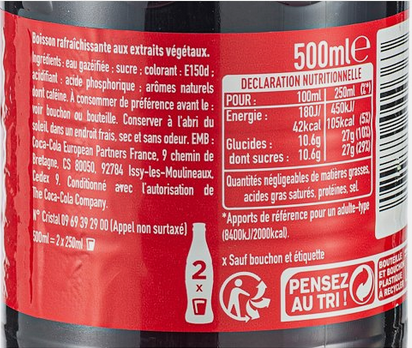
\includegraphics[scale=2]{Images/TP/TP6/Etiquette_coca.png}
  \end{center}
\end{doc}
 
%%%%
\newpage

%%%% documents
\begin{doc}{Utilisation d'une courbe d'étalonnage}
Une courbe d'étalonnage permet de relier deux grandeurs mesurables (par exemple la masse volumique et la concentration en masse). \\
L'idée est de fabriquer des \textcolor{red}{solutions étalons} avec des propriétés (masse volumique, concentration en masse, ...) que l'expérimentateur choisit puis mesure : ce sont les croix noires sur le graphique ci-dessous. Ensuite, on mesure une grandeur d'une solution inconnue (par exemple sa masse volumique) qu'on place sur la courbe d'étalonnage pour en déduire l'autre grandeur (par exemple sa concentration en masse) : c'est la croix bleue sur le graphique ci-dessous.
\begin{center}
    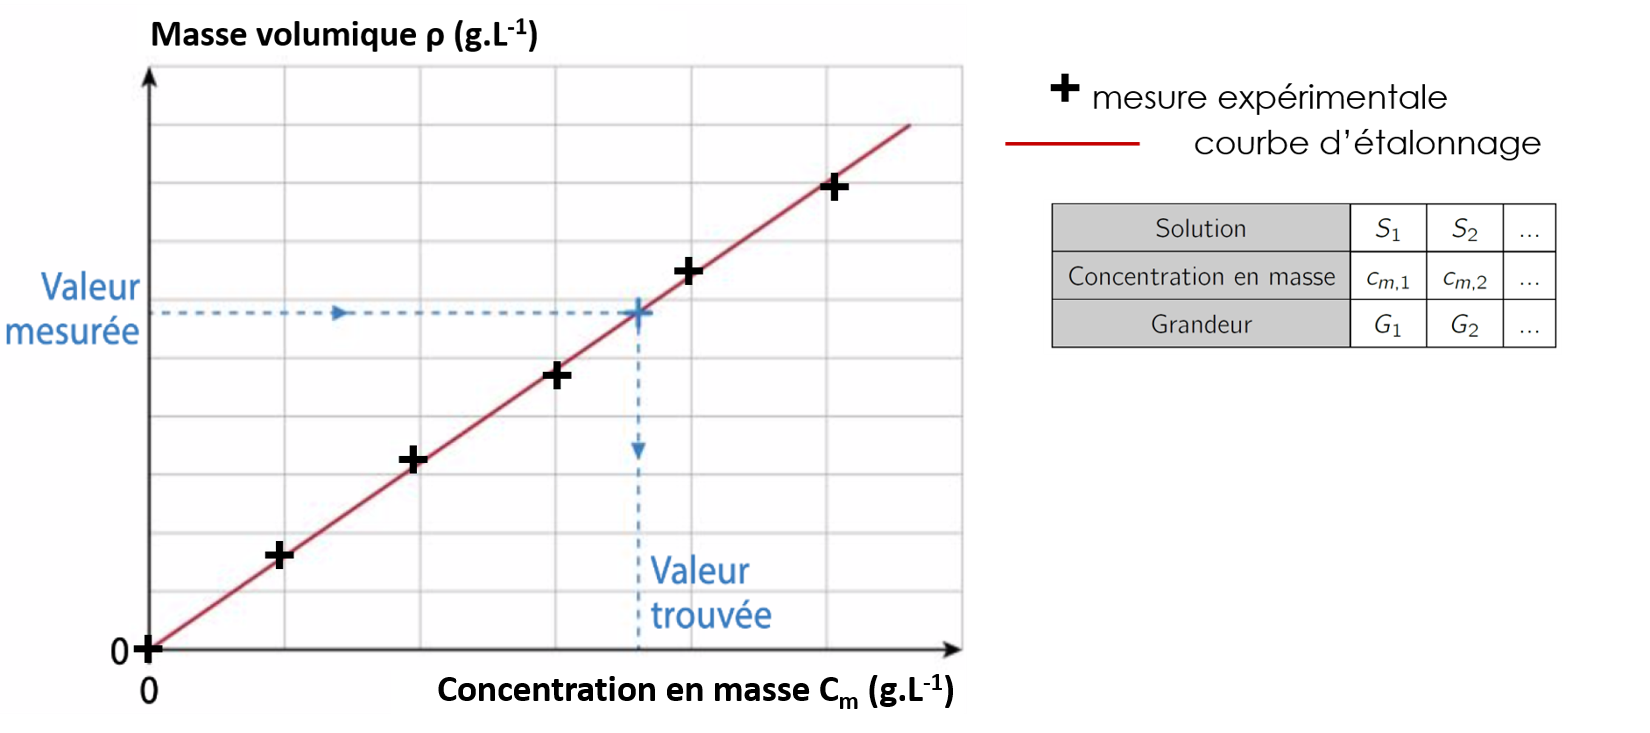
\includegraphics[scale=0.5]{Images/TP/TP6/Courbe_etalonnage.png}
\end{center}
On peut connaître la valeur recherchée soit par une lecture graphique, soit à l'aide d'une \textcolor{red}{courbe d'étalonnage} (courbe rouge sur le graphique ci-dessus) qui représente une modélisation mathématique du lien entre les deux grandeurs mesurées (une relation linéaire sur le grahique ci-dessus).
\end{doc}
%%%%
\begin{doc}{Protocole expérimental de préparation d'une solution aqueuse par dissolution}
\vspace{-0.8cm}
\begin{center}
    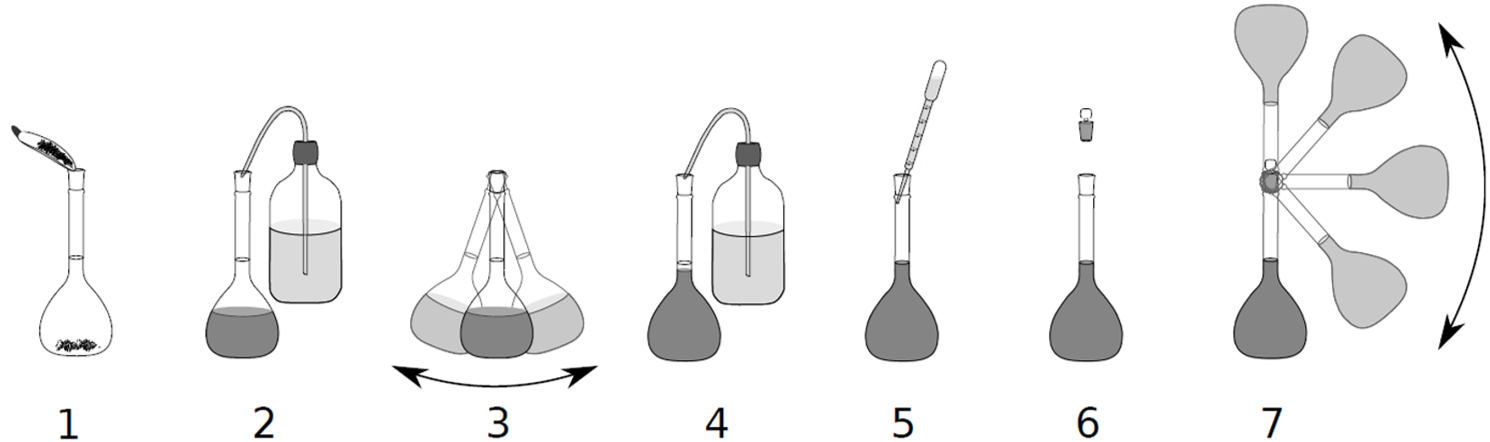
\includegraphics[scale=0.5]{Images/TP/TP6/Dissolution.png}
  \end{center}

\end{doc}

%%%%
\newpage
%%%%
\begin{large}
    \textbf{\textcolor{red}{\underline{Travail à réaliser :}}}
\end{large}
\\
\question{Télécharger le fichier \og \text{TP6\_Coca\_Resultats.xlsx}~\fg ~depuis l'ENT dans l'application "Espace Documentaire". Vous l'enregistrerez sur le bureau de votre session.}{~}{0}
\\
\question{Déterminer le solvant et au moins deux solutés dans le soda de marque bien connue.}{D'après le document \ref{doc:Coca}, le solvant est l'eau et deux solutés possibles sont : le sucre et le colorant E150d.}{0}
\\
\question{Déterminer la concentration en masse de sucre dans le soda à l'aide de l'étiquette de la bouteille de soda. On donnera le résultat en g.L$^{-1}$.}{On lit qu'il y a $m=10,6$~g de sucre pour $V=100$~mL de boisson soit une concentration en masse de sucre égale à $C_m= \frac{m}{V}=\frac{10,6}{0,100}=106$~g.L$^{-1}$.}{0}
\\
\question{\'{A} l'aide des explications et de l'expérience réalisée par le professeur, écrire votre protocole expérimental pour réaliser la dissolution d'une masse $m_{sucre}$ de sucre dans un volume $V$. \textbf{\underline{Attention de bien nommer la verrerie}} utilisée à chaque étape du protocole.}{Voici les étapes pour réaliser le protocole de dissolution :
\begin{enumerate}
    \item Peser la fiole jaugée, noter sa masse ;
    \item Mettre un entonnoir en plastique sur la fiole. Placer le tout sur la balance puis tarer la balance ;
    \item \`{A} l'aide d'une spatule, verser une masse $m_{sucre}$ de sucre dans l'entonnoir. Noter la valeur $m_{sucre}$ ;
    \item Rincer l'entonnoir à l'aide d'une pissette d'eau distillée ;
    \item Retirer l'entonnoir puis compléter jusqu'au 2/3 la fiole jaugée d'eau distillée ;
    \item Agiter la fiole pour dissoudre le sucre ;
    \item Compléter la fiole jaugée jusqu'au trait de jauge à l'aide d'une pipette pasteur ;
    \item Placer un bouchon et retourner plusieurs fois la fiole jaugée pour homogénéiser le mélange ;
    \item Peser la masse de l'ensemble \{fiole sans bouchon + solution d'eau sucrée\} et retirer la masse de la fiole jaugée pour en déduire la masse de solution d'eau sucrée ;
\end{enumerate}}{0}
%
\question{Calculer la masse de sucre à peser pour réaliser une solution d'eau sucrée de concentration en masse de sucre $C_{1}=55$~g.L$^{-1}$ de volume $V=100,0$~mL. \textbf{\underline{Expliciter clairement le détail du calcul.}}}{On cherche la masse $m_{sucre}$ telle que $C_m=55$~g.L$^{-1}$. D'après le cours et en utilisant les notations de la question, on sait que :
\begin{equation*}
    C_m = \frac{m_{sucre}}{V}
\end{equation*}
On en déduit donc :
\begin{equation*}
    m_{sucre} = C_m \times V = 55\times 0,100 = 5,5~\text{g}
\end{equation*}
On doit donc peser 5,5~g de sucre pour obtenir une telle solution.}{0}
\\
\question{Sans détailler les calculs, compléter le tableau suivant pour la masse de sucre :
\begin{center}
    \begin{tabular}{|c|C{0.15}|C{0.3}|C{0.1}|C{0.2}|}
    \hline
         Solution & Masse de sucre (en g) & Concentration en masse de sucre $C_m$ (en g.L$^{-1}$) & Volume (en mL) & Masse volumique $\rho$ (en g.L$^{-1}$) \\
         \hline
         $S_1$ & & 55 & 100,0 &\\
         \hline
         $S_2$ & & 75 & 100,0 & \\
         \hline
         $S_3$ & & 95 & 100,0 & \\
         \hline 
         $S_4$ & & 120 & 100,0 & \\
         \hline
    \end{tabular}
\end{center}}{\begin{center}
    \begin{tabular}{|c|C{0.15}|C{0.3}|C{0.1}|C{0.2}|}
    \hline
         Solution & Masse de sucre (en g) & Concentration en masse de sucre $C_m$ (en g.L$^{-1}$) & Volume (en mL) & Masse volumique $\rho$ (en g.L$^{-1}$)\\
         \hline
         $S_1$ & 5,5 & 55 & 100,0 & 1022 \\
         \hline
         $S_2$ & 7,5 & 75 & 100,0 & 1029 \\
         \hline
         $S_3$ & 9,5 & 95 & 100,0 & 1037 \\
         \hline 
         $S_4$ & 11,5 & 120 & 100,0 & 1046 \\
         \hline
    \end{tabular}
\end{center}}{0}

\question{Réaliser les solutions $S_1$ et $S_2$ pour les groupes A et les solutions $S_3$ et $S_4$ pour les groupes B.}{Travail en classe}{0}
\\
\question{Mesurer les masses volumiques de vos solutions et compléter le tableau de la question 6.}{Voir la question 4.}{0}
\\
\question{Reporter vos valeurs dans le tableur Excel. Tracer la courbe (ici une droite) d'étalonnage puis imprimer votre graphique que vous collerez dans votre compte-rendu.}{\begin{center}
    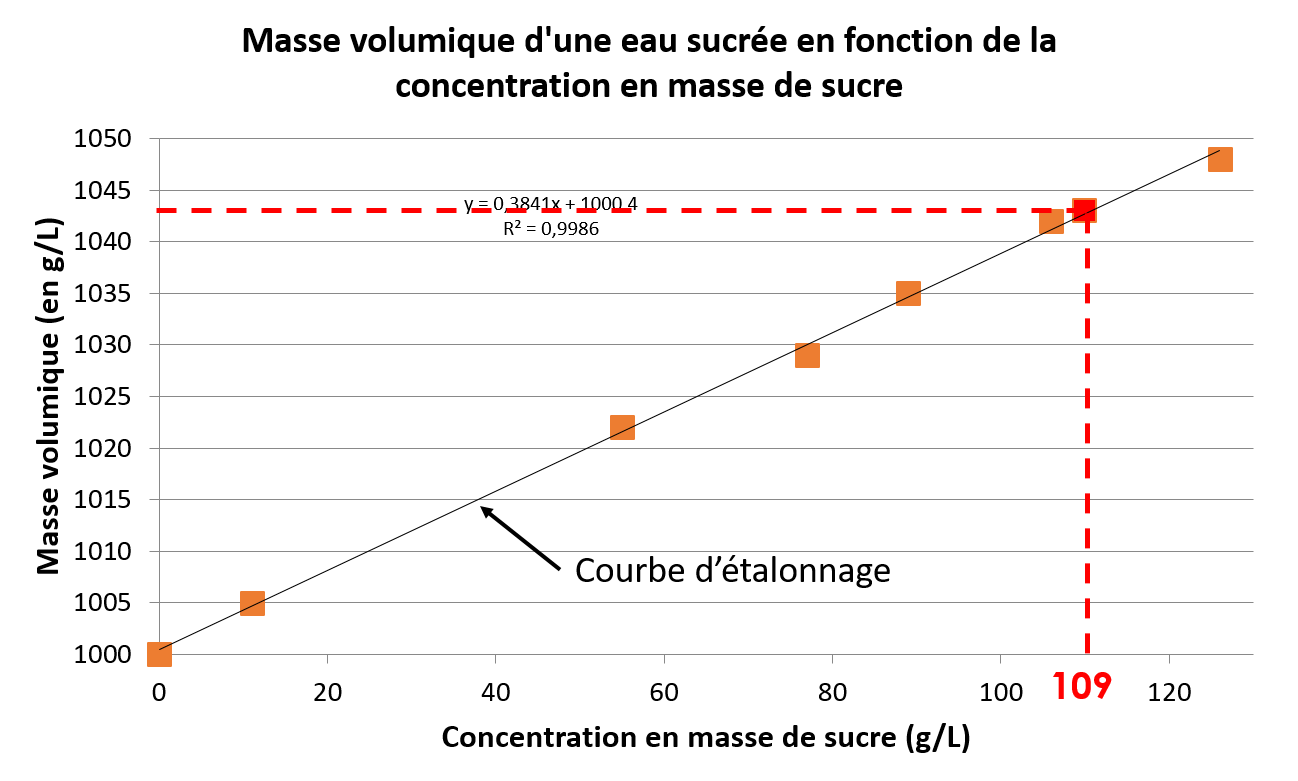
\includegraphics[scale=0.5]{Images/TP/TP6/Resultat_coca.png}
\end{center}}{0}
\question{Mesurer la masse volumique du soda, notée $\rho_{soda}$. Placer ce point sur votre courbe d'étalonnage.}{On verse 100,0~mL de soda dans une fiole jaugée dont on connaît la masse. On mesure la masse du liquide introduit et on détermine sa masse volumique. On trouve $\rho_{soda}=1043$~g.L$^{-1}$ qu'on place sur le graphique (carré rouge sur le graphique de la question 8).}{0}
\\
\question{En déduire la concentration en masse $C_{m}^{soda}$ de sucre dans le soda de marque bien connue.}{On en déduit par lecture graphique $C_{m}^{soda}=109$~g.L$^{-1}$.}{0}
\\
\question{Comparer la concentration en masse de sucre obtenue de vos mesures à celle donnée sur l'étiquette de la bouteille de soda. Proposer une explication sur la différence/la similitude entre votre résultat et celui attendu.}{On trouve une valeur très proche de celle donnée sur l'étiquette. Néanmoins nos mesures permettent de montrer que le résultat est légèrement différent (écart de 2,3\%). C'est normal puisque dans le soda, il y a d'autres ingrédients que le sucre (dont les concentrations en masse nous sont inconnues, secret d'entreprise !).}{0}
\\
\question{\textit{(Bonus)} L'OMS (Organisation Mondiale de la Santé) recommande de ne pas consommer plus de 100~g de sucre par jour pour rester en bonne santé, calculer combien de verres de $V=12,5$~cL du soda étudié un être humain peut consommer par jour.}{Un verre de 12,5~cL possède $m=C_m^{soda}\times V = 106\times 0,125=12,7$~g. Un être humain peut donc consommer environ 2 verres de soda par jour si son apport en sucre dans la journée provient uniquement du soda.}{0}
\\
\question{\textit{(Bonus)} Quelle serait la valeur de la masse volumique d'une solution si la concentration en masse de sucre était égale à $C_{m}=0$~g.L$^{-1}$ ? Vous donnerez le résultat en g.L$^{-1}$.}{On aurait une solution composée d'un volume de 100,0~mL d'eau distillée, sa masse volumique serait donc celle de l'eau soit $\rho_{eau}=1000$~g.L$^{-1}$.}{0}
%\begin{center}
%    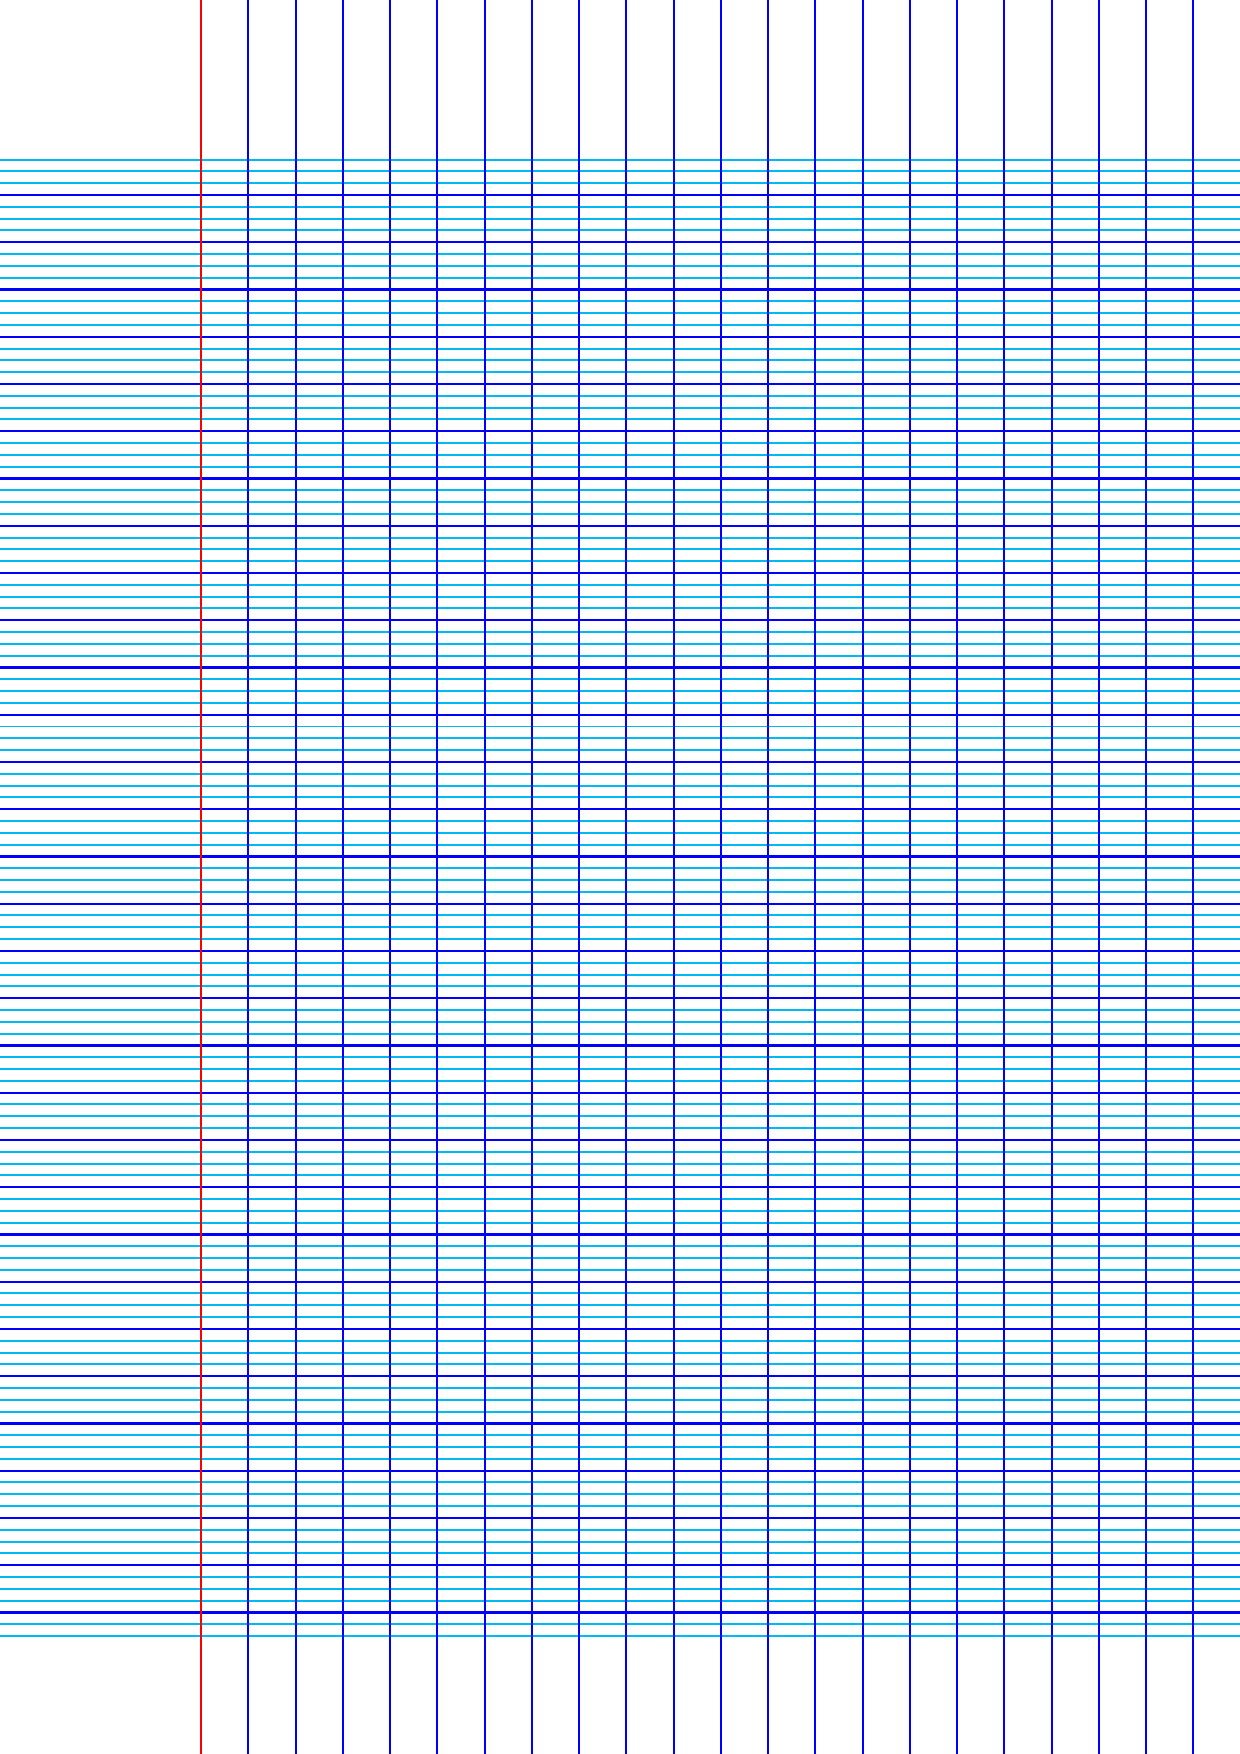
\includegraphics[scale=0.75]{Images/Feuilles/Grands_carreaux.pdf}
%\end{center}

%\begin{center}
 %   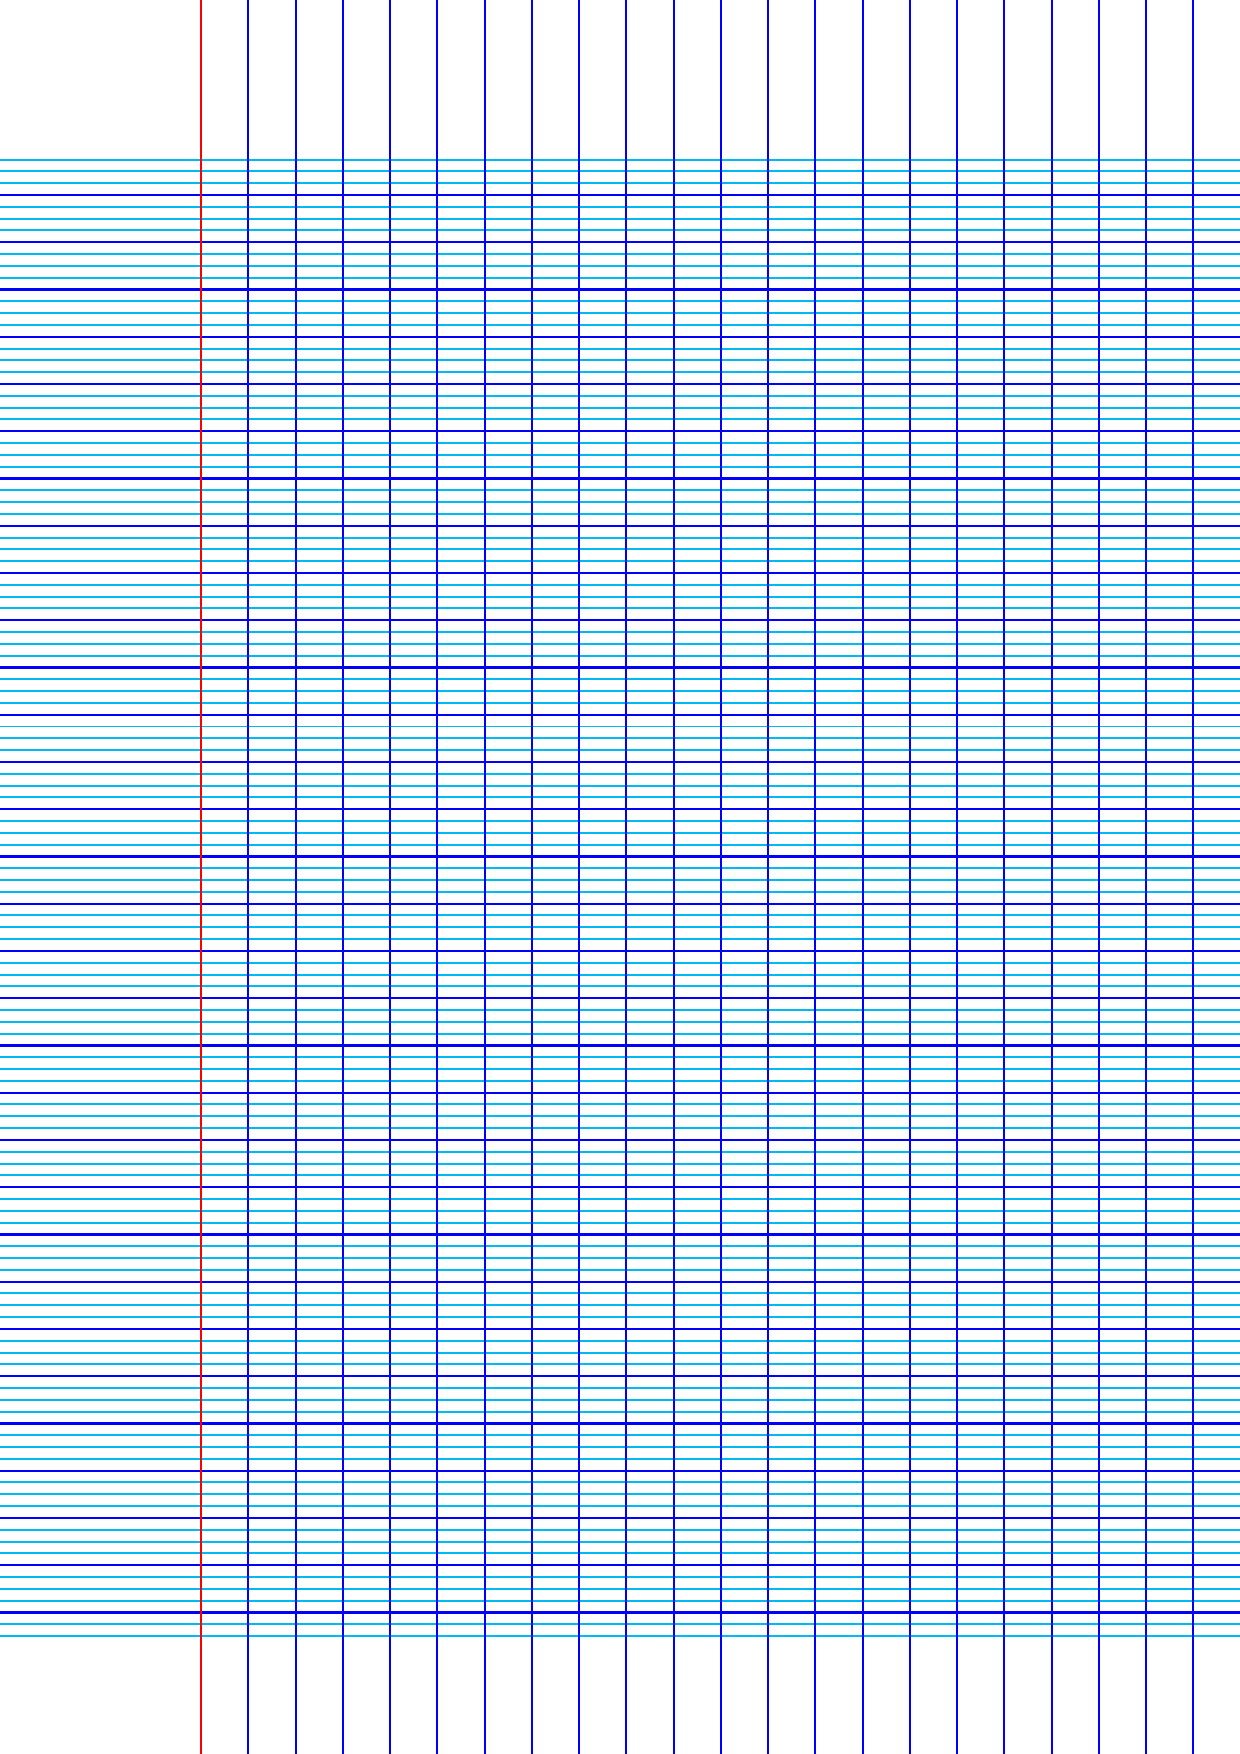
\includegraphics[scale=0.85]{Images/Feuilles/Grands_carreaux.pdf}
%\end{center}